\documentclass[tikz, border=10pt]{standalone}

\usetikzlibrary{arrows}

\begin{document}
	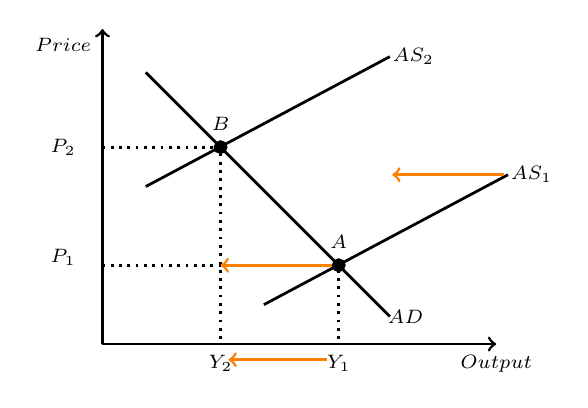
\begin{tikzpicture}[line width=1pt]
		\draw[->] (0, 0) -- (5, 0); % Горизонтальная линия
		\draw[->] (0, 0) -- (0, 4); % Вертикальная линия
	
		\draw[fill=black] (3, 1) circle (2pt);       % Точки P1-Y1
		\draw[fill=black] (1.5, 2.5) circle (2pt); % Точки P2-Y2
		
		\draw[dotted] (0, 1) -- (3, 1) -- (3, 0);              % Линии P1-Y1
		\draw[dotted] (0, 2.5) -- (1.5, 2.5) -- (1.5, 0); % Линии P2-Y2
		
		\draw (0.55, 3.45) -- (3.65, 0.35);
		\draw (0.55, 2) -- (3.65, 3.65);
		\draw (2.05, 0.5) -- (5.15, 2.15);
		
		\draw[->, color=orange] (2.92, 1) -- (1.5, 1);
		\draw[->, color=orange] (2.85, -0.2) -- (1.6, -0.2);
		\draw[->, color=orange] (5.1, 2.15) -- (3.68, 2.15);
	
	\begin{scriptsize}
		\draw (-0.5, 3.8) node {$Price$};
		\draw (5, -0.25) node {$Output$};
		
		\draw (-0.5, 1.1) node {$P_{1}$};
		\draw (-0.5, 2.5) node {$P_{2}$};
		
		\draw (3, -0.25) node {$Y_{1}$};
		\draw (1.5, -0.25) node {$Y_{2}$};
		
		\draw (1.5, 2.8) node {$B$};
		\draw (3, 1.3) node {$A$};
		\draw (3.85, 0.35) node {$AD$};
		\draw (3.95, 3.65) node {$AS_{2}$};
		\draw (5.45, 2.15) node {$AS_{1}$};
	\end{scriptsize}
\end{tikzpicture}
\end{document}